\documentclass{article}

\usepackage{defines}

\begin{document}

\tickettitle{9}{Полярная, цилиндрическая и сферическая системы координат.}

\define{полярной системы координат}

\begin{minipage}{0.6\linewidth}
	Полярной системой координат называется система, определяющими элементами которой являются:
	\begin{enumerate}
		\item{}точка $O$ --- полюс
		\item{}луч $O\rho$ из полюса --- полярная ось
		\item{}единица измереня длин на $O\rho$
		\item{}единица измерения углов $\varphi$ (rad)
		\item{}положительное направление отсчёта углов (против часовой стрелки)
	\end{enumerate}
\end{minipage}%
\begin{minipage}{0.4\linewidth}
	\centering
	\begin{tikzpicture}
		\filldraw (0,0) node[anchor=east] {$O$};
		\filldraw (1,2) circle (0.02) node[anchor=east] {$A$};
		\draw [dashed] (0,0)--(1,2);
		\draw [-latex] (0,0)--(2,0) node[above] {$\rho$};
		\draw [-latex] (1.5,0) arc (0:63:1.5) node[midway, above right] {$\varphi$};
	\end{tikzpicture}
	\captionof{figure}{Полярная система координат}\label{9:polar}
\end{minipage}

\define{полярных координат}

Рассмотрим полярную систему координат (\figref{9:polar}):
\begin{enumerate}
	\item{}$r$ --- полярный радиус:
	\begin{align*}
		 & r:=d(O,A) &  & r\in[0;+\infty)
	\end{align*}
	\item{}$\varphi$ --- полярный угол, $A\neq O$
	\begin{align*}
		 & \varphi:=\angle(O\rho,OA) &  & \varphi\in[0;2\pi)
	\end{align*}
\end{enumerate}

Полярные координаты точки $A(r,\varphi)$ --- упорядоченная пара чисел $(r,\varphi)$

Для точки $O$ координата $\varphi$ не определена.

\define{связи ДПСК и полярной СК}

\begin{minipage}{0.6\linewidth}
	\begin{enumerate}
		\item{}начало ДПСК совпадает с $O$
		\item{}$\vec{i}:\vec{i}\upuparrows O\rho\land|\vec{i}|=1$
		\item{}$\vec{j}:\vec{i}\perp\vec{j}\land|\vec{j}|=1\land O\vec{i}\vec{j}\text{ --- правая}$
		\item{}$O\vec{i}\vec{j}$ --- ДПСК
	\end{enumerate}

	полярная СК $\to$ ДПСК:
	\begin{align*}
		 & x=r\cos\varphi &  & y=r\sin\varphi
	\end{align*}

	ДПСК $\to$ полярная СК:
	\begin{align*}
		 & r=\sqrt{x^{2}+y^{2}} &  & \cos\varphi=\frac{x}{\sqrt{x^{2}+y^{2}}} &  & \sin\varphi=\frac{y}{\sqrt{x^{2}+y^{2}}}
	\end{align*}
\end{minipage}%
\begin{minipage}{0.4\linewidth}
	\centering
	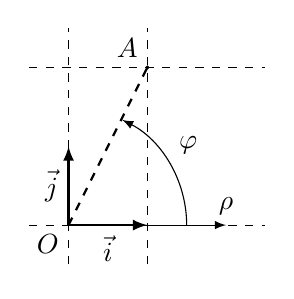
\begin{tikzpicture}
		\filldraw (0,0) node[anchor=east, yshift=-0.7em] {$O$};
		\filldraw (1,2) circle (0.02) node[anchor=east, yshift=0.7em] {$A$};
		\draw [dashed, thick] (0,0)--(1,2);
		\draw [-latex] (0,0)--(2,0) node[above] {$\rho$};
		\draw [-latex] (1.5,0) arc (0:63:1.5) node[midway, above right] {$\varphi$};
		\draw[-latex, thick] (0,0)--(1,0) node[midway,below] {$\vec{i}$};
		\draw[-latex, thick] (0,0)--(0,1) node[midway,left] {$\vec{j}$};
		\draw [dashed] (-0.5,0)--(2.5,0);
		\draw [dashed] (-0.5,2)--(2.5,2);
		\draw [dashed] (0,-0.5)--(0,2.5);
		\draw [dashed] (1,-0.5)--(1,2.5);
	\end{tikzpicture}
	\captionof{figure}{Полярная СК $\to$ ДПСК}
\end{minipage}

\pagebreak

\define{циллиндрической системы координат}

\begin{minipage}{0.6\linewidth}
	\begin{enumerate}
		\item{}В плоскости $\alpha$ введена полярная система координат с полюсом $O$ и осью $O\rho$
		\item{}Проведена ось $O\vec{k}\perp\alpha$
		\item{}Возьмём произвольную точку $M$ и $M'$ --- её проекцию на $\alpha$ вдоль $O\vec{k}$
		\item{}$(r,\varphi)$ --- полярные координаты $M'$
		\item{}$z:=\mes_{\vec{k}}\lvec{M'M}$
	\end{enumerate}
\end{minipage}%
\begin{minipage}{0.4\linewidth}
	\centering
	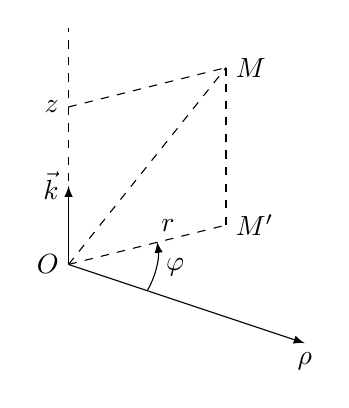
\begin{tikzpicture}
		\filldraw (0,0) node[anchor=east] {$O$};
		\filldraw (2,0.5) node[anchor=west] {$M'$};
		\filldraw (2,2.5) node[anchor=west] {$M$};
		\filldraw (0,2) node[anchor=east] {$z$};
		\draw [-latex] (0,0)--(3,-1) node[below] {$\rho$};
		\draw [-latex] (0,0)--(0,1) node[left] {$\vec{k}$};
		\draw [dashed] (0,0)--(0,3);
		\draw [dashed] (0,0)--(2,2.5);
		\draw [dashed] (0,0)--(2,0.5) node[left=1.5em] {$r$};
		\draw [dashed] (2,0.5)--(2,2.5);
		\draw [dashed] (0,2)--(2,2.5);
		\draw [-latex] (1,-0.333) arc (-30:7:1) node[midway, right] {$\varphi$};
	\end{tikzpicture}
	\captionof{figure}{Циллиндрическая СК}
\end{minipage}

$(r,\varphi,z)$ --- циллиндрические координаты точки $M$ (только в таком порядке).

\define{связи ДПСК и циллиндрической СК}

\begin{minipage}{0.6\linewidth}
	\begin{enumerate}
		\item{}Начало ДПСК совпадает с $O$
		\item{}$\vec{i}:\vec{i}\upuparrows O\rho\land|\vec{i}|=1$
		\item{}$\vec{k}:\vec{k}\upuparrows O\vec{k}\land|\vec{k}|=1$
		\item{}$\vec{j}:|\vec{j}|=1\land O\vec{i}\vec{j}\vec{k}\text{ --- правая}$
	\end{enumerate}

	циллиндрическая $\to$ ДПСК
	\begin{align*}
		 & x=r\cos\varphi &  & y=r\cos\varphi &  & z=z
	\end{align*}

	ДПСК $\to$ циллиндрическая
	\begin{align*}
		 & r=\sqrt{x^{2}+y^{2}} &  & \cos\varphi=\frac{x}{\sqrt{x^{2}+y^{2}}} \\
		 & z=z                  &  & \sin\varphi=\frac{y}{\sqrt{x^{2}+y^{2}}}
	\end{align*}
\end{minipage}%
\begin{minipage}{0.4\linewidth}
	\centering
	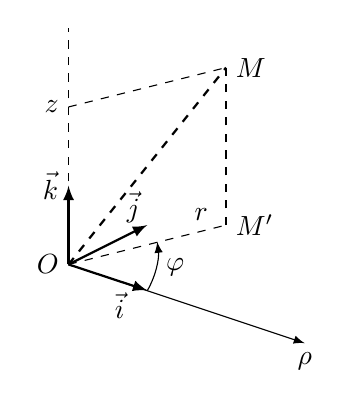
\begin{tikzpicture}
		\filldraw (0,0) node[anchor=east] {$O$};
		\filldraw (2,0.5) node[anchor=west] {$M'$};
		\filldraw (2,2.5) node[anchor=west] {$M$};
		\filldraw (0,2) node[anchor=east] {$z$};
		\draw [-latex] (0,0)--(3,-1) node[below] {$\rho$};
		\draw [-latex, thick] (0,0)--(0,1) node[left] {$\vec{k}$};
		\draw [dashed] (0,0)--(0,3);
		\draw [dashed, thick] (0,0)--(2,2.5);
		\draw [dashed] (0,0)--(2,0.5) node[above left=-0.2em, xshift=-0.5em] {$r$};
		\draw [dashed] (2,0.5)--(2,2.5);
		\draw [dashed] (0,2)--(2,2.5);
		\draw [-latex] (1,-0.333) arc (-30:7:1) node[midway, right] {$\varphi$};
		\draw [-latex, thick] (0,0)--(1,-0.33) node[below, xshift=-1em, yshift=0.3em] {$\vec{i}$};
		\draw [-latex, thick] (0,0)--(1, 0.5) node[above, xshift=-0.5em, yshift=-0.3em] {$\vec{j}$};
	\end{tikzpicture}
	\captionof{figure}{Циллиндрическая СК $\to$ ДПСК}
\end{minipage}

\pagebreak

\define{сферической системы координат}

\begin{minipage}{0.6\linewidth}
	\begin{enumerate}
		\item{}В плоскости $\alpha$ введена полярная система координат с полюсом $O$ и осью $O\rho$
		\item{}Проведена ось $O\vec{k}\perp\alpha$
		\item{}Возьмём произвольную точку $M$ и $M'$ --- её проекцию на $\alpha$ вдоль $O\vec{k}$
		\item{}$(r,\varphi)$ --- полярные координаты $M'$
		\item{}$R:=d(O,M)$, $R\in[0;+\infty)$, $R$ --- сферический радиус
		\item{}$\varphi:=\angle(O\rho, OM')$, $\varphi\in[0;2\pi)$, $\varphi$ --- долгота
		\item{}$\psi:=\angle(OM,OM')$, $\psi\in\left[-\cfrac{\pi}{2};\cfrac{\pi}{2}\right]$, $\psi$ --- широта
	\end{enumerate}
\end{minipage}%
\begin{minipage}{0.4\linewidth}
	\centering
	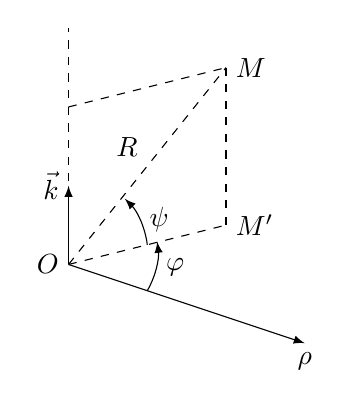
\begin{tikzpicture}
		\filldraw (0,0) node[anchor=east] {$O$};
		\filldraw (2,0.5) node[anchor=west] {$M'$};
		\filldraw (2,2.5) node[anchor=west] {$M$};
		\draw [-latex] (0,0)--(3,-1) node[below] {$\rho$};
		\draw [-latex] (0,0)--(0,1) node[left] {$\vec{k}$};
		\draw [dashed] (0,0)--(0,3);
		\draw [dashed] (0,0)--(2,2.5) node[midway, above left] {$R$};
		\draw [dashed] (0,0)--(2,0.5);
		\draw [dashed] (2,0.5)--(2,2.5);
		\draw [dashed] (0,2)--(2,2.5);
		\draw [-latex] (1,-0.333) arc (-30:7:1) node[midway, right] {$\varphi$};
		\draw [-latex] (1,0.25) arc (7:45:1) node[midway, right] {$\psi$};
	\end{tikzpicture}
	\captionof{figure}{Сферическая СК}
\end{minipage}

$(r,\varphi,\psi)$ --- сферические координаты точки $M$ (только в таком порядке).

\define{связи ДПСК и сферической СК}

\begin{minipage}{0.6\linewidth}
	\begin{enumerate}
		\item{}Начало ДПСК совпадает с $O$
		\item{}$\vec{i}:\vec{i}\upuparrows O\rho\land|\vec{i}|=1$
		\item{}$\vec{k}:\vec{k}\upuparrows O\vec{k}\land|\vec{k}|=1$
		\item{}$\vec{j}:|\vec{j}|=1\land O\vec{i}\vec{j}\vec{k}\text{ --- правая}$
	\end{enumerate}

	сферическая $\to$ циллиндрическая $\to$ ДПСК
	\begin{align*}
		 & r=R\cos\psi &  & x=r\cos\varphi=R\cos\psi\cos\varphi \\
		 & z=R\sin\psi &  & y=r\cos\varphi=R\cos\psi\sin\varphi
	\end{align*}
\end{minipage}%
\begin{minipage}{0.4\linewidth}
	\centering
	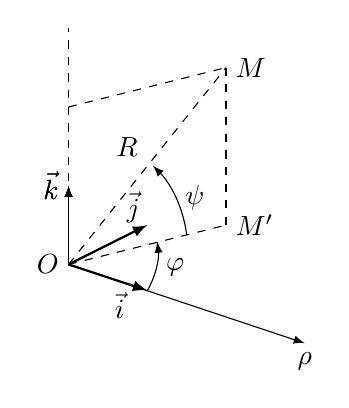
\begin{tikzpicture}
		\filldraw (0,0) node[anchor=east] {$O$};
		\filldraw (2,0.5) node[anchor=west] {$M'$};
		\filldraw (2,2.5) node[anchor=west] {$M$};
		\draw [-latex] (0,0)--(3,-1) node[below] {$\rho$};
		\draw [-latex] (0,0)--(0,1) node[left] {$\vec{k}$};
		\draw [dashed] (0,0)--(0,3);
		\draw [dashed] (0,0)--(2,2.5) node[midway, above left] {$R$};
		\draw [dashed] (0,0)--(2,0.5);
		\draw [dashed] (2,0.5)--(2,2.5);
		\draw [dashed] (0,2)--(2,2.5);
		\draw [-latex] (1,-0.333) arc (-30:7:1) node[midway, right] {$\varphi$};
		\draw [-latex] (1.5,0.375) arc (7:45:1.5) node[midway, right] {$\psi$};
		\draw [-latex, thick] (0,0)--(1,-0.33) node[below, xshift=-1em, yshift=0.3em] {$\vec{i}$};
		\draw [-latex, thick] (0,0)--(1, 0.5) node[above, xshift=-0.5em, yshift=-0.3em] {$\vec{j}$};
		\draw [-latex] (0,0)--(0,1) node[left] {$\vec{k}$};
	\end{tikzpicture}
	\captionof{figure}{Сферическая СК $\to$ ДПСК}
\end{minipage}

\end{document}
